\documentclass{article}
\usepackage[utf8]{inputenc}
\usepackage[margin=1in]{geometry}
\usepackage{amsmath, amssymb, amsthm, graphicx, float}
\usepackage{subfig, subfloat}
\allowdisplaybreaks

\title{Automatic Test Generation via ML: Draft Documentation}
\author{Arjun Jauhari}
\date{10 December 2015}

\begin{document}

\maketitle

\begin{figure}[H]
\centering
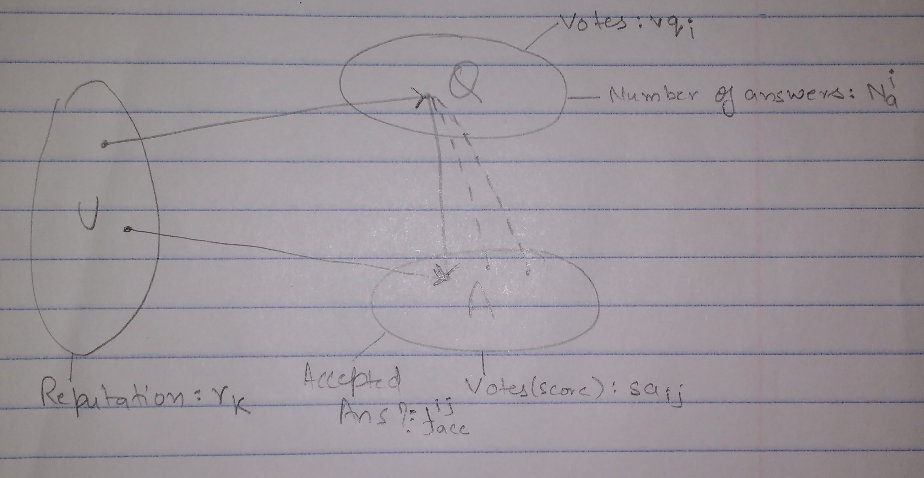
\includegraphics[width=14cm]{overview.png}
\caption{Overview}
\label{fig1:overview}
\end{figure}

\section*{Subscripts}
\begin{itemize}
    \item $i$ is subscript for question.
    \item $j$ is subscript for answer.
    \item $k$ is subscript for user.
\end{itemize}
\section*{Notations}
\begin{enumerate}
    \item $u_k$: Quality measure of the $k$th user.
    \item $q_i$: Quality measure of the $i$th question.
    \item $va_{ij}$: Normalized votes corresponding to $j$th answer of $i$th question. \\
        Calculated as: $va_{ij} = \frac{|sa_{ij}|}{\sum_{j} |sa_{ij}|}$ \\
        where $sa_{ij}$ is the actual votes(score) read from data dump.
    \item $a_{ijk}$: Quality measure of $a_{ij}$th answer given by the $k$th user.
    \item $f_{acc}^{ij}$: Boolean flag telling if this answer was Accepted, read from data dump.
    \item $r_k$: Reputation of the $k$th user, read from data dump.
    \item $N_{a}^{i}$: Number of answer to $i$th question, read from data dump.
    \item $vq_{i}$: Number of votes to $i$th question, read from data dump.
\end{enumerate}

\section*{Equations}
Below equations model the relation/dependence between
the above defined parameters. \\
\begin{enumerate}
    \item $a_{ijk} = f_a(u_k, q_i, va_{ij}, f_{acc}^{ij})$
    \item $u_k = f_u(\{a_{ijk}\}_{ij}, q_i, r_k)$ , where $\{a_{ijk}\}_{ij}$
        is set of all answers by user k
    \item $q_i = f_q(u_k, N_{a}^{i}, vq_i, \{a_{ijk}\}_{jk})$, where $\{a_{ijk}\}_{jk}$
        is set of all answers to $i$th question
\end{enumerate}

\section*{Status}
Currently, the model is very simple with $va_{ij} = \frac{|sa_{ij}|}{\sum_{j} |sa_{ij}|}$, where $sa_{ij}$ is the actual votes(score) read from data dump.\\
and $a_{ijk} = w_1*u_k + w_2*q_i + w_3*va_{ij} + w_4*f_{acc}^{ij}$ \\
\\
As of now weights $w_1, w_2, w_4$ are 0 and $w_3$ is 1, so $a_{ijk} = va_{ij}$ \\
\\
User quality is being modeled as: $u_k \sim \mathcal{N} (mean(\{a_{ijk}\}_{ij}), Var(\{a_{ijk}\}_{ij}))$ \\
\\
Question quality is still not modeled.

\end{document}

